\section{Persönlicher Rubic}

\subsection{Abrizz: Balance}

\begin{figure}[H]
	\centering
	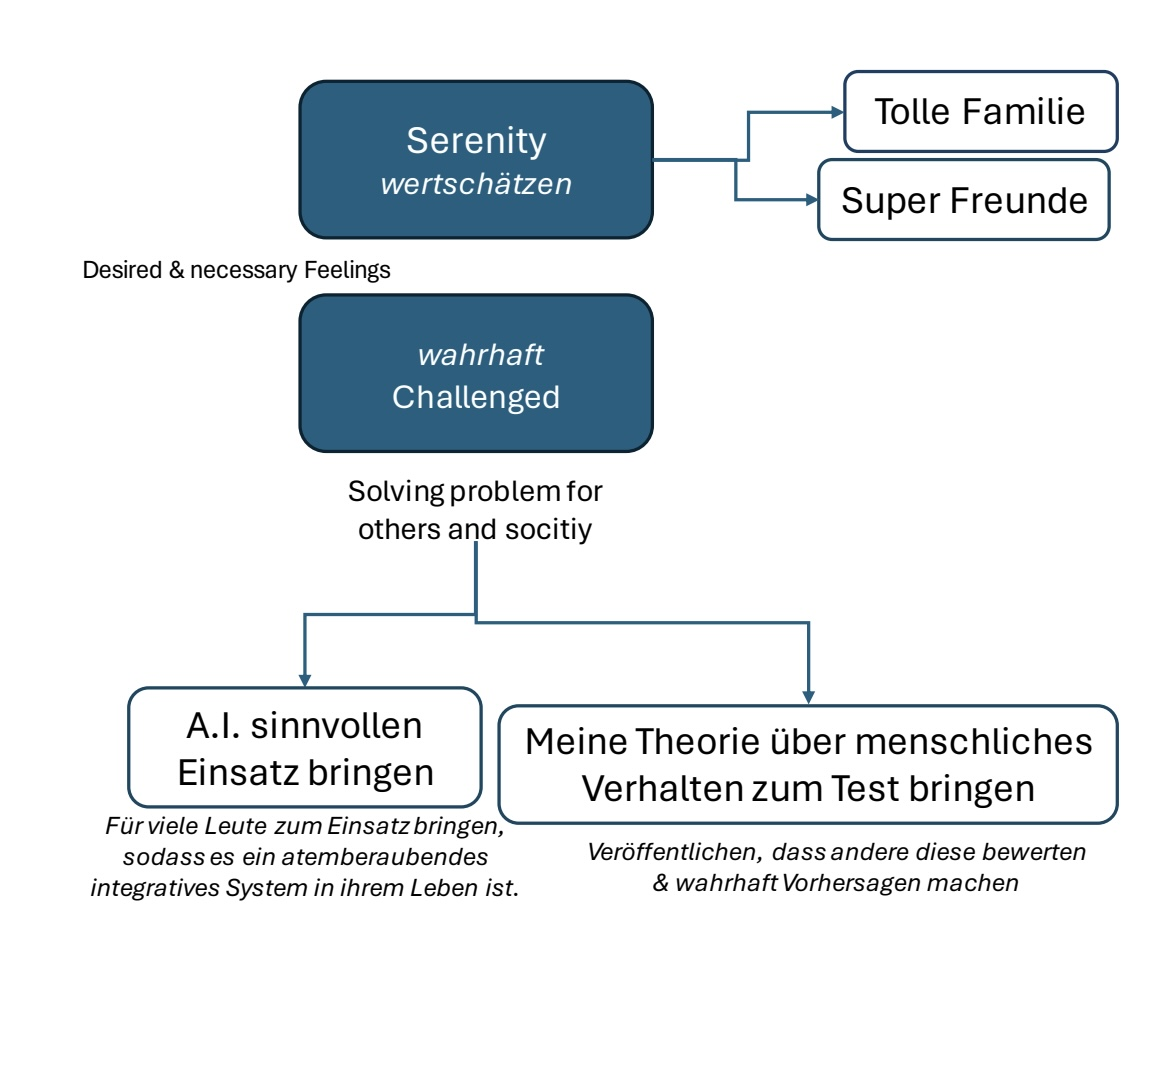
\includegraphics[scale = 0.2]{attachment/chapter_OWN/Scc009}
	\caption{Desired and necessary  feelings}
\end{figure}

Die Balance zwischen zwei Gefühlen strebe ich für mein Leben an:
\begin{itemize}
    \item Serenity wertzuschätzen 
    \item und wahrhaft Challenged  sich zu fühlen
\end{itemize}

\subsection{Wertschätzen Serenity}

Die Überlegung dahinter ist, dass die Maximierung des stimulierenden Gefühls "Challenged" mit der Ausrichtung auf die Zukunft (Dopamin) keine langfristig erreichbare Basis für mich ist, weil ich auf die Zielsetzung für \textit{Serentiy} nicht zu verzichten:
\begin{itemize}
    \item Eine großartige Familie
    \item und tolle Freunde.
\end{itemize}
Um das Gefühl von Herausforderung ohne größere Einbußen des allgemeinen Wohlbefindens zu erreichen, sehe ich die Balance mit den Zielen für das Gefühl von  \textit{Serenity} als unabdingbar an.\\

Mir ist dabei bewusst, dass einige Herausforderungen leichter zu erreichen sind, indem die gesetzten Ziele zurückgestellt oder aufgegeben werden. Meine Hoffnung und gleichzeitig gesetzte Herausforderung ist jedoch, einen Weg zu finden, Herausforderungen zu setzen und zu erreichen, ohne dabei auf Familie und Freude zu verzichten. 

\subsection{Wahrhaft Challenged}
Bei dem Gefühl \textit{Challenged} geht es vorallem um die Phase bis zu Bewähltigung der gesetzten Herausforderungen. Die bisherige Erkenntnis ist, dass wenn das Ziel erreicht ist, automatisch \textit{Serentiy} einsetzt.\\

Die Option kurz vor der Erreichung keine Kraft mehr hineinzustecken, ist keine Option. Das Problem der eigenen gefühlten Unglaubwürdigkeit sorgt dafür, dass beim nächsten Mal die Phase bis zur Erreichung der Herausforderungen nicht so stimmulierend ist, weil man selbst annimt, dass diese nicht erreicht wird. Und das Gefühl von einer wahrhaft erreichten Herausforderung, ist unschlagbar.\\

Für mich ist verbirgt sich hinter dem Gefühl \textit{Challenged}, dass besonders für mich stimulierend ist, wenn \textit{Herausforderungen für andere oder die Gesellschaft} gelöst werden. Für jemand anders oder representive für die Gesellschaft ein Problem zu lösen, was auch für mich herausfordernd ist, macht den Stimmulus aus.\\

Die Herausforderungen können sich  logischerweise ändern und weiterentwickeln. Zwei der drei Schwerpunkt sind als so formuliert, dass sie helfen, Entscheidungen und Projekt zu beeinflussen, sodass sich ständig gefragt wird, ob man sich in die richtig Richtung bewegt.\\

\paragraph{A.I. Technologie zum sinnvollen Einsatz bringen}
Was damit gemeint ist, dass eine große Anzahl von Personen davon einen Mehrwert erhalten. Zum einen soll damit angestrebt werden, dass die Anerkennung durch den Einsatz dieser anspruchsvollen Technologie herrüht und zum anderen, dass ein Problem gelöst wird, was den Menschen von Bedeutung ist.\\

Die Herausforderung für mich ist, dass ich die drei Gebiete von Data Science zum Einsatz bringen kann und diese Einsatz aller drei, eine so spannende \textit{challenged} Gefühl mir gibt.\\

Um aber nicht im klein-klein zu versacken, ist der erste Teil entscheiden: Es ist nur eine wahre Herausforderung, wenn ich dies für hinreichend viele Personen umsetzen kann.

Hier sind die korrigierten Abschnitte:

\paragraph{Veröffentlichung Meiner Theorie}
In mir keimt der Gedanke, dass ich einen oder mehrere Startpunkte gefunden habe, von denen es interessant und stimulierend wäre, eine Theorie aufzubauen, die einen Ansatz bietet, einen Teil menschlichen Verhaltens vorherzusagen, ähnlich wie es in der Physik möglich ist.

Damit ich hier nicht im klein-klein versinke, sind zwei Punkte entscheidend:
\begin{itemize}
    \item Die Vorhersagen müssen im Experiment überprüft werden.
    \item Die Theorie muss veröffentlicht werden.
\end{itemize}

\paragraph{Einen Weg für Herausforderungen und Familie finden}
Wie bereits erwähnt, besteht die Annahme, dass sich, wenn man sich ausschließlich auf Herausforderungen konzentriert, diese leichter erreichen lassen. In meiner eigenen Selbstwahrnehmung sehe ich, dass ich ohne ein solides Fundament von Freunden und Familie nicht das volle Potenzial des Gefühls von "Challenged" ausschöpfen kann, weil ich im Detail steckenbleibe.

Das Ziel besteht darin, einen Weg im Lösungsraum zu finden, der es mir ermöglicht, beides zu erreichen: Herausforderungen anzugehen, die mir das stimulierende Gefühl von "Challgend" geben, und gleichzeitig meinen persönlichen Bedarf an einer glücklichen Familie und Freunden zu decken.